\section{LO3: Design Principles vs. Data}

\subsection{Data Preprocessing for Effective Visualization}
The Gapminder dataset presents itself in a fairly clean and well-structured format, which is conducive for effective visualization. However, for datasets that are not as pristine, a series of critical preprocessing steps would be necessary. For the Gapminder dataset, these hypothetical steps could include:

\begin{itemize}
  \item \textbf{Handling Missing Values:} Inspecting the dataset for any missing data points. Although the Gapminder dataset has negligible missing values, in a less ideal scenario, methods like imputation or exclusion of incomplete records would be considered based on the context and the amount of missing data.
  
  \item \textbf{Data Normalization:} For datasets where economic indicators like GDP per capita vary significantly over time due to inflation, normalization or adjustment for purchasing power parity would be essential. The Gapminder dataset's GDP values are already adjusted for inflation, but in other cases, this step would ensure temporal comparability of economic data \cite{GDPCapitaV25}.
  
  \item \textbf{Data Transformation:} Applying transformations such as logarithmic scaling to handle skewed distributions, especially for variables like GDP per capita that can span several orders of magnitude. This step, is also relevant for the Gapminder dataset, as seen in Figure \ref{fig:lo3_scatterplot}.
  
  \item \textbf{Categorization and Binning:} Grouping continuous variables into categories can be useful for certain types of analyses. For example, categorizing countries into income brackets or creating age groups from continuous age data would be pertinent. The Gapminder dataset, however, does not necessitate such binning for most analyses due to its focus on country-level aggregated indicators.
\end{itemize}

In sum, while the Gapminder dataset's clean state allows for a more straightforward visualization process, these preprocessing steps are fundamental practices for handling less refined datasets and ensuring that the subsequent visualizations accurately represent the underlying data narratives.

\subsection{Visualization Design Choices}
The visualization design is directly influenced by the nature of the preprocessed data. For the Gapminder dataset, we chose:
\begin{itemize}
  \item \textbf{Scatter Plots:} To illustrate correlations, such as between life expectancy and GDP per capita, highlighting global disparities seen in Figure \ref{fig:lo3_scatterplot}. Using the logarithmic scale for GDP per capita allows for a more effective comparison across countries with diverse economic backgrounds.
  \item \textbf{Bar Charts:} For demographic comparisons, like population distribution across continents. The bar chart in Figure \ref{fig:lo3_barchart} shows the population distribution across continents in 2007.
  \item \textbf{Color Schemes:} Employing distinct hues to differentiate continents, enhancing interpretability.
\end{itemize}

Each choice is geared towards making complex global data comprehensible and engaging for the audience.

\begin{figure}[h]
    \centering
    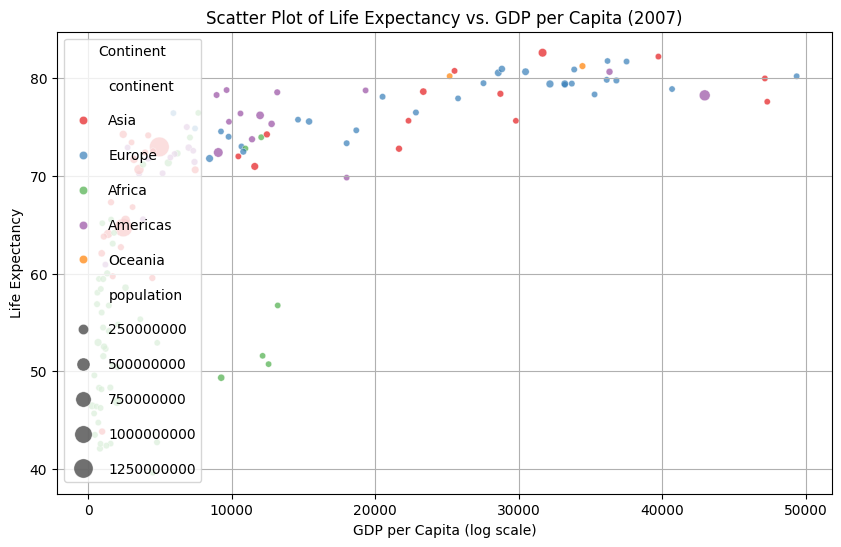
\includegraphics[width=0.8\textwidth]{images/plots/lo3_scatterplot.png} 
    \caption{Scatter Plot of Life Expectancy vs. GDP per Capita (2007): A Visualization Reflecting Design Choices.}
    \label{fig:lo3_scatterplot}
\end{figure}

\begin{figure}[h]
    \centering
    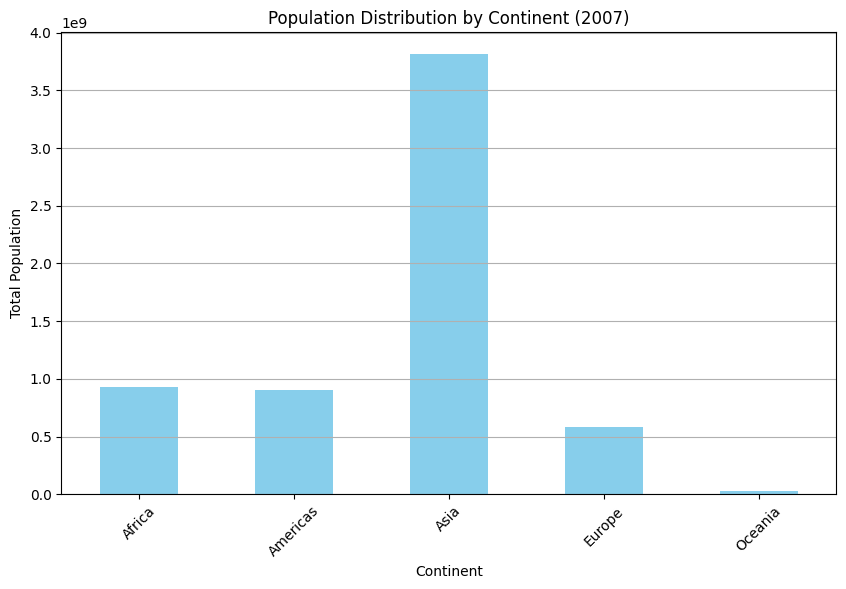
\includegraphics[width=0.8\textwidth]{images/plots/lo3_barplot.png} 
    \caption{Bar Chart of Population Distribution Across Continents (2007): A Visualization Reflecting Design Choices.}
    \label{fig:lo3_barchart}
\end{figure}

\subsection{Integration of Data and Design}
The design decisions, from chart types to color choices, are made to enhance the dataset's storytelling. For instance, the scatter plot’s logarithmic scale for GDP per capita allows for an effective comparison across countries with diverse economic backgrounds. This approach facilitates a deeper understanding of the interplay between economic status and health outcomes globally.

\subsection{Challenges and Solutions}
One significant challenge was presenting a vast range of GDP values in a single visualization. The solution was to implement a logarithmic scale, making it easier to discern patterns and outliers in countries' economic data. This choice underscores the importance of adapting visualization techniques to suit the data's nature and the intended message.